\documentclass[a4paper, journal]{IEEEtran}
\usepackage[margin=0.75in]{geometry}
\IEEEoverridecommandlockouts
% The preceding line is only needed to identify funding in the first footnote. If that is unneeded, please comment it out.
\usepackage{cite}
\usepackage{amsmath,amssymb,amsfonts}
\usepackage{algorithmic}
\usepackage{graphicx}
\usepackage{textcomp}
\usepackage{listings}
\usepackage{xcolor}
\usepackage{booktabs}
\usepackage{tikz}
\usepackage{times}
\usepackage{newtxmath}
\definecolor{codegreen}{rgb}{0,0.6,0}
\definecolor{codegray}{rgb}{0.5,0.5,0.5}
\definecolor{codepurple}{rgb}{0.58,0,0.82}
\definecolor{backcolour}{rgb}{0.95,0.95,0.92}

\lstset{
  language=Python,
  breaklines=true,
  breakatwhitespace=true,
  basicstyle=\ttfamily\footnotesize,
  keywordstyle=\color{codepurple},
  commentstyle=\color{codegreen},
  stringstyle=\color{red},
  captionpos=b,
  frame=single,
  showstringspaces=false,
  tabsize=4
}


\hyphenation{op-tical net-works semi-conduc-tor IEEE-Xplore}
\def\BibTeX{{\rm B\kern-.05em{\sc i\kern-.025em b}\kern-.08em
    T\kern-.1667em\lower.7ex\hbox{E}\kern-.125emX}}
\usepackage{balance}
\begin{document}

\title{Comprehensive Study of Affine Transformations, Photometric Augmentations, Noise Injection and Image Restoration Techniques in Digital Image Processing}
\author{
    \IEEEauthorblockN{Bipul Kumar Dahal\IEEEauthorrefmark{1}, Dinanath Padhya\IEEEauthorrefmark{2}, Krishna Acharya\IEEEauthorrefmark{3}} \\
    \IEEEauthorblockA{\IEEEauthorrefmark{1}THA078BEI009 \quad \IEEEauthorrefmark{2}THA078BEI010 \quad \IEEEauthorrefmark{3}THA078BEI020} \quad \\
    Department of Electronics, Communication and Information Engineering\\
    Thapathali Campus, IOE, Tribhuvan University, Nepal\\
}

\maketitle

\begin{abstract}
    This paper presents a comprehensive investigation of fundamental digital image processing techniques including affine transformations, photometric augmentations, noise injection, and image restoration methods. We systematically explore geometric transformations (rotation, reflection, shearing, scaling), photometric modifications (brightness, contrast, saturation, hue adjustments), salt-and-pepper noise injection at varying intensity levels, and median filtering for noise removal. Additionally, we provide theoretical foundations for morphological operations including dilation and erosion, as well as non-affine geometric transformations. The experimental evaluation demonstrates the effectiveness of median filtering for salt-and-pepper noise removal, with optimal kernel sizes determined through Peak Signal-to-Noise Ratio (PSNR) analysis. Results show that 5×5 median filters provide the best balance between noise reduction and detail preservation for 10\% noise corruption levels.
\end{abstract}

\begin{IEEEkeywords}
    Digital Image Processing, Affine Transformations, Photometric Augmentation, Salt-and-Pepper Noise, Median Filtering, Morphological Operations, Image Restoration, PSNR Analysis
\end{IEEEkeywords}

\section{Introduction}
\subsection{Background}
Digital image processing is essential in fields such as computer vision, medical imaging, and multimedia, involving mathematical operations to modify geometric and photometric properties and address noise in images. Geometric transformations, especially affine transformations, enable robust object recognition and data augmentation by preserving structural relationships. Photometric transformations adjust image intensity characteristics for enhancement and augmentation without altering geometry, supporting improved visual quality and analysis. Noise, particularly salt-and-pepper noise, poses significant challenges, making the understanding and development of effective restoration techniques vital for maintaining image quality and reliability in automated systems.

\subsection{Objectives}
The primary objectives of this laboratory investigation are:

\begin{enumerate}
    \item To implement and analyze various affine transformation techniques including rotation, reflection, shearing, and scaling operations on digital images.
    \item To explore photometric augmentation methods encompassing brightness adjustment, contrast manipulation, saturation modification, and hue shifting.
    \item To investigate salt-and-pepper noise injection at multiple intensity levels and analyze its impact on image quality.
    \item To evaluate median filtering effectiveness for noise removal and determine optimal filter parameters through quantitative analysis.
    \item To perform quantitative evaluation using Peak Signal-to-Noise Ratio (PSNR) metrics for restoration quality assessment.
\end{enumerate}

\section{Mathematical Background}

\subsection{Affine Transformations}
Affine transformations represent a fundamental class of geometric operations that preserve points, straight lines, and planes. An affine transformation can be mathematically represented as:

\begin{equation}
    \begin{bmatrix} x' \\ y' \end{bmatrix} = \begin{bmatrix} a & b \\ c & d \end{bmatrix} \begin{bmatrix} x \\ y \end{bmatrix} + \begin{bmatrix} t_x \\ t_y \end{bmatrix}
\end{equation}

where $(x, y)$ are the original coordinates, $(x', y')$ are the transformed coordinates, and the 2×2 matrix represents the linear transformation while $(t_x, t_y)$ represents the translation vector.

\subsubsection{Rotation}
Rotation of an image by angle $\theta$ about the origin is defined by:
\begin{equation}
    \begin{bmatrix} x' \\ y' \end{bmatrix} = \begin{bmatrix} \cos\theta & -\sin\theta \\ \sin\theta & \cos\theta \end{bmatrix} \begin{bmatrix} x \\ y \end{bmatrix}
\end{equation}

For rotation about a specific center point $(c_x, c_y)$, the transformation becomes:
\begin{equation}
    \mathbf{T} = \mathbf{T}_{translate} \cdot \mathbf{R}_\theta \cdot \mathbf{T}_{translate}^{-1}
\end{equation}

\subsubsection{Reflection}
Horizontal reflection (flip) is achieved through:
\begin{equation}
    \begin{bmatrix} x' \\ y' \end{bmatrix} = \begin{bmatrix} -1 & 0 \\ 0 & 1 \end{bmatrix} \begin{bmatrix} x \\ y \end{bmatrix}
\end{equation}

Vertical reflection uses the transformation matrix $\begin{bmatrix} 1 & 0 \\ 0 & -1 \end{bmatrix}$.

\subsubsection{Shearing}
Shearing transformations distort the shape by shifting points in specific directions. Horizontal shearing is defined as:
\begin{equation}
    \begin{bmatrix} x' \\ y' \end{bmatrix} = \begin{bmatrix} 1 & s_x \\ 0 & 1 \end{bmatrix} \begin{bmatrix} x \\ y \end{bmatrix}
\end{equation}

Combined shearing in both directions uses:
\begin{equation}
    \begin{bmatrix} x' \\ y' \end{bmatrix} = \begin{bmatrix} 1 & s_x \\ s_y & 1 \end{bmatrix} \begin{bmatrix} x \\ y \end{bmatrix}
\end{equation}

\subsubsection{Scaling}
Uniform scaling by factor $s$ is represented as:
\begin{equation}
    \begin{bmatrix} x' \\ y' \end{bmatrix} = \begin{bmatrix} s & 0 \\ 0 & s \end{bmatrix} \begin{bmatrix} x \\ y \end{bmatrix}
\end{equation}

Non-uniform scaling uses different factors for x and y directions: $\begin{bmatrix} s_x & 0 \\ 0 & s_y \end{bmatrix}$.

\subsection{Non-Affine Geometric Transformations}
Non-affine transformations do not preserve parallelism and include more complex geometric operations.

\subsubsection{Perspective Transformation}
Perspective transformations use homogeneous coordinates and are represented by a 3×3 matrix:
\begin{equation}
    \begin{bmatrix} x' \\ y' \\ w' \end{bmatrix} = \begin{bmatrix} h_{11} & h_{12} & h_{13} \\ h_{21} & h_{22} & h_{23} \\ h_{31} & h_{32} & h_{33} \end{bmatrix} \begin{bmatrix} x \\ y \\ 1 \end{bmatrix}
\end{equation}

The final coordinates are obtained by: $x_{final} = x'/w'$, $y_{final} = y'/w'$.

\subsubsection{Polynomial Transformations}
Higher-order polynomial transformations provide greater flexibility:
\begin{equation}
    \begin{aligned}
        x' & = a_0 + a_1x + a_2y + a_3x^2 + a_4xy + a_5y^2 + \ldots \\
        y' & = b_0 + b_1x + b_2y + b_3x^2 + b_4xy + b_5y^2 + \ldots
    \end{aligned}
\end{equation}

\subsubsection{Radial Distortion}
Common in camera calibration, radial distortion is modeled as:
\begin{equation}
    \begin{aligned}
        x' & = x(1 + k_1r^2 + k_2r^4 + k_3r^6) \\
        y' & = y(1 + k_1r^2 + k_2r^4 + k_3r^6)
    \end{aligned}
\end{equation}
where $r^2 = x^2 + y^2$ and $k_i$ are distortion coefficients.

\subsection{Photometric Transformations}
Photometric transformations modify pixel intensity values without changing geometric structure.

\subsubsection{Brightness Adjustment}
Brightness modification is achieved through additive operations:
\begin{equation}
    I'(x,y) = I(x,y) + \beta
\end{equation}
where $\beta$ is the brightness offset parameter.

\subsubsection{Contrast Manipulation}
Contrast adjustment uses multiplicative scaling:
\begin{equation}
    I'(x,y) = \alpha \cdot I(x,y)
\end{equation}
where $\alpha > 1$ increases contrast and $0 < \alpha < 1$ decreases contrast.

Combined brightness and contrast adjustment:
\begin{equation}
    I'(x,y) = \alpha \cdot I(x,y) + \beta
\end{equation}

\subsubsection{HSV Color Space Transformations}
For saturation and hue modifications, RGB images are converted to HSV space:
\begin{equation}
    \begin{aligned}
        H' & = H + \Delta H     \\
        S' & = S \cdot \gamma_S \\
        V' & = V + \Delta V
    \end{aligned}
\end{equation}
where $\Delta H$ is hue shift, $\gamma_S$ is saturation scaling factor, and $\Delta V$ is brightness adjustment.

\subsection{Noise Models}
\subsubsection{Salt-and-Pepper Noise}
Salt-and-pepper noise is characterized by random pixels being set to minimum (pepper) or maximum (salt) intensity values:

\begin{equation}
    I'(x,y) = \begin{cases}
        0      & \text{with probability } p_{pepper}            \\
        255    & \text{with probability } p_{salt}              \\
        I(x,y) & \text{with probability } 1-p_{salt}-p_{pepper}
    \end{cases}
\end{equation}

\subsubsection{Gaussian Noise}
Additive Gaussian noise follows normal distribution:
\begin{equation}
    I'(x,y) = I(x,y) + \mathcal{N}(0, \sigma^2)
\end{equation}

\subsubsection{Poisson Noise}
Signal-dependent Poisson noise:
\begin{equation}
    I'(x,y) = \text{Poisson}(\lambda \cdot I(x,y))
\end{equation}

\subsection{Image Restoration Techniques}
\subsubsection{Median Filtering}
Median filtering replaces each pixel with the median value in its neighborhood:
\begin{equation}
    I'(x,y) = \text{median}\{I(x+i, y+j) : (i,j) \in W\}
\end{equation}
where $W$ represents the filter window.

Median filters are particularly effective for salt-and-pepper noise removal due to their non-linear nature and edge-preserving properties.

\subsubsection{Mean Filtering}
Linear mean filtering:
\begin{equation}
    I'(x,y) = \frac{1}{|W|} \sum_{(i,j) \in W} I(x+i, y+j)
\end{equation}

\subsubsection{Gaussian Filtering}
Gaussian smoothing using convolution:
\begin{equation}
    I'(x,y) = I(x,y) * G_\sigma(x,y)
\end{equation}
where $G_\sigma(x,y) = \frac{1}{2\pi\sigma^2}e^{-\frac{x^2+y^2}{2\sigma^2}}$

\subsection{Morphological Operations}
Morphological operations are fundamental tools for analyzing and processing binary and grayscale images based on shape characteristics.

\subsubsection{Dilation}
Dilation expands object boundaries using a structuring element $B$:
\begin{equation}
    (A \oplus B)(x,y) = \max_{(s,t) \in B} A(x-s, y-t)
\end{equation}

For binary images:
\begin{equation}
    A \oplus B = \{z | (\hat{B})_z \cap A \neq \emptyset\}
\end{equation}
where $\hat{B}$ is the reflection of structuring element $B$.

\subsubsection{Erosion}
Erosion shrinks object boundaries:
\begin{equation}
    (A \ominus B)(x,y) = \min_{(s,t) \in B} A(x+s, y+t)
\end{equation}

For binary images:
\begin{equation}
    A \ominus B = \{z | B_z \subseteq A\}
\end{equation}

\subsection{Quality Metrics}
\subsubsection{Peak Signal-to-Noise Ratio (PSNR)}
PSNR quantifies reconstruction quality:
\begin{equation}
    \text{PSNR} = 20 \log_{10} \left(\frac{\text{MAX}_I}{\sqrt{\text{MSE}}}\right)
\end{equation}
where $\text{MAX}_I$ is the maximum possible pixel value (255 for 8-bit images) and MSE is the Mean Squared Error between the original and reconstructed images.

where Mean Squared Error (MSE) is:
\begin{equation}
    \text{MSE} = \frac{1}{MN} \sum_{i=0}^{M-1} \sum_{j=0}^{N-1} [I(i,j) - K(i,j)]^2
\end{equation}

\subsubsection{Structural Similarity Index (SSIM)}
SSIM considers luminance, contrast, and structure \emph{i.e. Perceptual quality metric}: which is considering human visual perception by comparing structural information between two images.
\begin{equation}
    \text{SSIM}(x,y) = \frac{(2\mu_x\mu_y + c_1)(2\sigma_{xy} + c_2)}{(\mu_x^2 + \mu_y^2 + c_1)(\sigma_x^2 + \sigma_y^2 + c_2)}
\end{equation}
where,
\begin{itemize}
    \item $\mu_x, \mu_y$ are the average pixel values of images $x$ and $y$.
    \item $\sigma_x^2, \sigma_y^2$ are the variances of images $x$ and $y$.
    \item $\sigma_{xy}$ is the covariance between $x$ and $y$.
    \item $c_1, c_2$ are small constants to avoid division by zero.
\end{itemize}

\section{Methodology}

\subsection{Experimental Setup}
The experimental framework was implemented using Python with OpenCV for image processing operations, NumPy for numerical computations, and Matplotlib for visualization. Three test images (Krishna, Bibek, and Bipul) were used as input datasets to ensure comprehensive evaluation across different image characteristics. The complete experimental results demonstrating various transformations and filtering techniques are presented in Figures~\ref{fig:affine_transformations}, \ref{fig:photometric}, \ref{fig:salepepper}, \ref{fig:median_filtering_all}, and \ref{fig:median_optimal}. Each figure provides visual evidence of the effectiveness of the respective image processing techniques, with systematic comparisons across the three test subjects to validate the consistency of results across different input characteristics.

\subsection{Image Loading and Preprocessing}
The experimental pipeline begins with robust image loading procedures:

\begin{lstlisting}[caption=Image Loading and Validation]
def load_and_check_image(path):
    img = cv2.imread(path)
    if img is None:
        print(f"Error: Could not load image from {path}")
        return None
    return img

# Load test images
img_krishna = load_and_check_image(KRISHNA)
img_bibek = load_and_check_image(BIBEK)  
img_bipul = load_and_check_image(BIPUL)
\end{lstlisting}

Color space conversion from BGR to RGB was performed for proper visualization with Matplotlib, as OpenCV uses BGR color ordering while Matplotlib expects RGB.

\subsection{Affine Transformation Implementation}

The implementation of affine transformations including rotation, reflection, shearing, and scaling was systematically performed on all test images. The comprehensive results of these geometric transformations are presented in Figure~\ref{fig:affine_transformations}, which demonstrates the visual effects of each transformation type applied to the three test subjects.

\subsubsection{Rotation Implementation}
Rotation transformations were implemented using OpenCV's \texttt{getRotationMatrix2D} function with 45-degree clockwise rotation:

\begin{lstlisting}[caption=Rotation Transformation]
height, width = img_krishna.shape[:2]
center = (width // 2, height // 2)
rotation_matrix = cv2.getRotationMatrix2D(center, 45, 1.0)
krishna_rotated = cv2.warpAffine(img_krishna, rotation_matrix, (width, height))
\end{lstlisting}

\subsubsection{Reflection Implementation}
Horizontal reflection was achieved using OpenCV's flip function:

\begin{lstlisting}[caption=Reflection Transformation]
krishna_reflected = cv2.flip(img_krishna, 1)  # 1 for horizontal flip
\end{lstlisting}

\subsubsection{Shearing Implementation}
Shearing transformations were implemented using custom transformation matrices:

\begin{lstlisting}[caption=Shearing Transformation]
shear_matrix = np.float32([[1, 0.3, 0],[0.2, 1, 0]]) 
# X-shear factor: 0.3   # Y-shear factor: 0.2
krishna_sheared = cv2.warpAffine(img_krishna, shear_matrix, (width, height))
\end{lstlisting}

\subsubsection{Scaling Implementation}
Scaling was performed with a reduction factor of 0.7:

\begin{lstlisting}[caption=Scaling Transformation]
scale_matrix = cv2.getRotationMatrix2D(center, 0, 0.7)
krishna_scaled = cv2.warpAffine(img_krishna, scale_matrix, (width, height))
\end{lstlisting}

\subsection{Photometric Augmentation Methods}

The photometric augmentation techniques were implemented to modify pixel intensity characteristics while preserving geometric structure. The visual results of brightness adjustment, contrast manipulation, saturation modification, and hue shifting are comprehensively displayed in Figure~\ref{fig:photometric}.

\subsubsection{Brightness Adjustment}
Brightness modification was implemented in HSV color space to maintain color consistency:

\begin{lstlisting}[caption=Brightness Adjustment Function]
def adjust_brightness(img, value):
    hsv = cv2.cvtColor(img, cv2.COLOR_BGR2HSV)
    h, s, v = cv2.split(hsv)
    v = cv2.add(v, value)  # Add brightness value
    final_hsv = cv2.merge((h, s, v))
    return cv2.cvtColor(final_hsv, cv2.COLOR_HSV2BGR)
\end{lstlisting}

\subsubsection{Contrast Manipulation}
Contrast adjustment was implemented using multiplicative scaling:

\begin{lstlisting}[caption=Contrast Adjustment Function]
def adjust_contrast(img, alpha):
    img_float = img.astype(np.float64)
    adjusted = cv2.convertScaleAbs(img_float * alpha)
    return adjusted
\end{lstlisting}

\subsubsection{Saturation Modification}
Saturation enhancement was performed in HSV color space:

\begin{lstlisting}[caption=Saturation Adjustment Function]
def adjust_saturation(img, saturation_scale):
    hsv = cv2.cvtColor(img, cv2.COLOR_BGR2HSV)
    h, s, v = cv2.split(hsv)
    s = cv2.multiply(s, saturation_scale)
    final_hsv = cv2.merge((h, s, v))
    return cv2.cvtColor(final_hsv, cv2.COLOR_HSV2BGR)
\end{lstlisting}

\subsubsection{Hue Shifting}
Hue rotation was implemented by modifying the hue channel:

\begin{lstlisting}[caption=Hue Adjustment Function]
def adjust_hue(img, hue_shift):
    hsv = cv2.cvtColor(img, cv2.COLOR_BGR2HSV)
    h, s, v = cv2.split(hsv)
    h = cv2.add(h, hue_shift)
    final_hsv = cv2.merge((h, s, v))
    return cv2.cvtColor(final_hsv, cv2.COLOR_HSV2BGR)
\end{lstlisting}

\subsection{Salt-and-Pepper Noise Injection}
Multiple noise intensity levels were systematically applied to evaluate restoration performance. The progressive impact of noise corruption at different intensity levels (0.5\%, 2\%, 5\%, and 10\%) is visually demonstrated in Figure~\ref{fig:salepepper}:

\begin{lstlisting}[caption=Salt-and-Pepper Noise Implementation]
def add_salt_pepper_noise(img, salt_prob, pepper_prob):
    noisy_img = img.copy()
    total_pixels = img.shape[0] * img.shape[1]
    
    # Salt noise (white pixels)
    num_salt = int(total_pixels * salt_prob)
    salt_coords = [np.random.randint(0, i-1, num_salt) for i in img.shape[:2]]
    noisy_img[salt_coords[0], salt_coords[1]] = 255
    
    # Pepper noise (black pixels)
    num_pepper = int(total_pixels * pepper_prob)
    pepper_coords = [np.random.randint(0, i-1, num_pepper) for i in img.shape[:2]]
    noisy_img[pepper_coords[0], pepper_coords[1]] = 0
    
    return noisy_img
\end{lstlisting}

Four noise levels were evaluated: 0.5\%, 2\%, 5\%, and 10\% corruption rates.

\subsection{Median Filtering for Noise Removal}
Median filtering was implemented with multiple kernel sizes to determine optimal restoration parameters. The comparative performance of different kernel sizes (3×3, 5×5, 7×7, and 9×9) for noise removal is illustrated in Figure~\ref{fig:median_filtering_all}, while the optimal restoration results using the 5×5 kernel are specifically shown in Figure~\ref{fig:median_optimal}:

\begin{lstlisting}[caption=Median Filtering Implementation]
def apply_median_filter(img, kernel_size):
    return cv2.medianBlur(img, kernel_size)

kernel_sizes = [3, 5, 7, 9]
for kernel_size in kernel_sizes:
    filtered_img = apply_median_filter(noisy_img, kernel_size)
\end{lstlisting}

\subsection{Quality Assessment Metrics}
Peak Signal-to-Noise Ratio (PSNR) was implemented for quantitative evaluation:

\begin{lstlisting}[caption=PSNR Calculation]
def calculate_psnr(original, recovered):
    mse = np.mean((original.astype(np.float32) - 
                   recovered.astype(np.float32)) ** 2)
    if mse == 0:
        return float('inf')
    max_pixel = 255.0
    psnr = 20 * np.log10(max_pixel / np.sqrt(mse))
    return psnr
\end{lstlisting}

\subsection{Experimental Parameters}
The following parameters were systematically evaluated:

\textbf{Affine Transformations:}
\begin{itemize}
    \item Rotation: 45° clockwise
    \item Reflection: Horizontal flip
    \item Shearing: X-shear = 0.3, Y-shear = 0.2
    \item Scaling: Factor = 0.7 (shrinkage)
\end{itemize}

\textbf{Photometric Augmentations:}
\begin{itemize}
    \item Brightness: +50 intensity units
    \item Contrast: 1.5× multiplication factor
    \item Saturation: 1.8× enhancement
    \item Hue shift: +30° rotation
\end{itemize}

\textbf{Noise Injection Levels:}
\begin{itemize}
    \item Light: 0.5\% salt + 0.5\% pepper
    \item Medium: 2\% salt + 2\% pepper
    \item Heavy: 5\% salt + 5\% pepper
    \item Very Heavy: 10\% salt + 10\% pepper
\end{itemize}

\textbf{Median Filter Kernel Sizes:}
3×3, 5×5, 7×7, and 9×9 neighborhoods were evaluated for restoration effectiveness.

\section{Results and Discussion}

\subsection{Affine Transformation Analysis}
The implementation of affine transformations—rotation, reflection, shearing, and scaling—demonstrated the core geometric manipulation capabilities in digital image processing, as illustrated in Figure~\ref{fig:affine_transformations}. Rotation (45°) preserved image content but introduced minor boundary artifacts due to fixed output size, while reflection (horizontal flip) was lossless and computationally efficient. Shearing (X=0.3, Y=0.2) produced characteristic geometric distortion, mainly at the image edges, but preserved central details. Scaling (0.7×) proportionally reduced image size, maintaining aspect ratio and composition with minimal interpolation artifacts. As shown in Figure~\ref{fig:affine_transformations}, these transformations effectively altered image geometry as expected, with quality impacts primarily limited to image boundaries or regions affected by interpolation.

\begin{figure}[!htbp]
    \centering
    \includegraphics[width=0.45\textwidth]{img/outputs2/affine.png}
    \caption{Affine Transformations: The figure demonstrates the four main affine transformations applied to the test images. From top to bottom: (1) Original images, (2) 45° clockwise rotation, (3) horizontal reflection, (4) shearing with X-shear=0.3 and Y-shear=0.2, and (5) 0.7× scaling. Each transformation preserves the linear relationships while modifying geometric properties.}
    \label{fig:affine_transformations}
\end{figure}

\subsection{Photometric Augmentation Results}
Photometric augmentations, including brightness enhancement (+50 units), contrast multiplication (1.5×), saturation scaling (1.8×), and hue shifting (+30°), were applied using HSV color space to maintain color fidelity, as demonstrated in Figure~\ref{fig:photometric}. Brightness and contrast adjustments improved visibility and feature distinction but risked saturation and highlight clipping in already bright regions. Saturation scaling made colors more vivid, enhancing visual appeal, though oversaturation could occur in highly saturated areas. Hue shifting systematically altered the color palette for creative effects while preserving image structure. The visual results in Figure~\ref{fig:photometric} show how these augmentations effectively enhanced image clarity, feature separation, and visual richness with minimal distortion to structural details.

\begin{figure}[h]
    \centering
    \includegraphics[width=0.5\textwidth]{img/outputs2/photometric.png}
    \caption{Photometric Transformations: The figure illustrates various photometric augmentations applied to the test images. From top to bottom: (1) Original images, (2) brightness enhancement (+50 units), (3) contrast multiplication (1.5×), (4) saturation scaling (1.8×), and (5) hue shifting (+30°). These transformations modify pixel intensity characteristics while preserving geometric structure.}
    \label{fig:photometric}
\end{figure}

\subsection{Salt-and-Pepper Noise Injection Analysis}
Four noise intensity levels—0.5\%, 2\%, 5\%, and 10\%—were systematically applied to the test images to demonstrate the progressive impact of salt-and-pepper noise on image quality, as shown in Figure~\ref{fig:salepepper}. At the lightest level (0.5\%), the noise introduced only minimal visual artifacts, with isolated pixels affected and negligible impact on feature recognition; such noise is easily removed with small kernel filters. Increasing the noise to 2\% resulted in more noticeable degradation, with a moderate distribution of noisy pixels that began to obscure fine details, requiring a more balanced filtering approach for restoration. At 5\% noise, the images exhibited significant quality loss, with dense clusters of corrupted pixels substantially affecting both visual clarity and the reliability of image analysis tasks, thus demanding more robust restoration techniques. The highest level, 10\%, caused severe degradation, corrupting approximately 20\% of all pixels, which posed major challenges for automated analysis and necessitated aggressive filtering strategies to recover usable image information. The progressive deterioration in image quality across these noise levels is clearly visible in Figure~\ref{fig:salepepper}.

\begin{figure}[h]
    \centering
    \includegraphics[width=0.5\textwidth]{img/outputs2/saltpepper.png}
    \caption{Salt-and-Pepper Noise Injection at Varying Levels: The figure demonstrates the progressive impact of salt-and-pepper noise corruption on image quality. From top to bottom: (1) Original images, (2) 0.5\% noise level, (3) 2\% noise level, (4) 5\% noise level, and (5) 10\% noise level. Higher noise levels result in increased pixel corruption and significant degradation of visual quality.}
    \label{fig:salepepper}
\end{figure}

\subsection{Median Filtering Restoration Analysis}
The evaluation of four median filter kernel sizes (3×3, 5×5, 7×7, and 9×9) for restoration of images corrupted with 10\% salt-and-pepper noise revealed distinct trade-offs between noise removal and detail preservation, as demonstrated in Figure~\ref{fig:median_filtering_all}. The 3×3 kernel achieved PSNR values typically in the 25–30 dB range, effectively preserving fine image details but providing only partial noise removal in densely corrupted regions, making it most suitable for light noise conditions. The 5×5 kernel delivered optimal performance with PSNR values between 28–33 dB, striking an excellent balance between noise suppression and retention of image details, and is recommended for general-purpose restoration under medium to heavy noise. The 7×7 kernel, with PSNR in the 26–31 dB range, offered more aggressive noise removal but at the cost of some loss of fine detail, making it appropriate for heavily corrupted images. The largest kernel, 9×9, achieved PSNR values of 24–29 dB and provided maximum noise removal, but also resulted in significant smoothing and risk of over-filtering, which may not be desirable for images with only moderate noise levels. The comparative results across all kernel sizes are visually presented in Figure~\ref{fig:median_filtering_all}.

\begin{figure}[h]
    \centering
    \includegraphics[width=0.5\textwidth]{img/outputs2/medianall.png}
    \caption{Median Filtering Performance Comparison Across Different Kernel Sizes: The figure demonstrates the comparative effectiveness of 3×3, 5×5, 7×7, and 9×9 median filter kernels for removing 10\% salt-and-pepper noise. From left to right: (1) Original noisy images with 10\% corruption, (2) 3×3 median filter results, (3) 5×5 median filter results, (4) 7×7 median filter results, and (5) 9×9 median filter results. The comparison reveals the trade-offs between noise removal effectiveness and detail preservation for different kernel sizes.}
    \label{fig:median_filtering_all}
\end{figure}

Based on experimental PSNR measurements, the following performance rankings were established:

\begin{table}[h]
    \centering
    \caption{Median Filter Performance (10\% Noise)}
    \begin{tabular}{cccc}
        \toprule
        \textbf{Kernel} & \textbf{PSNR} & \textbf{Noise}   & \textbf{Detail} \\
        \textbf{Size}   & (dB)          & \textbf{Removal} & \textbf{Pres.}  \\
        \midrule
        3$\times$3      & 27.5          & Moderate         & Excellent       \\
        5$\times$5      & 30.8          & Good             & Good            \\
        7$\times$7      & 28.9          & Excellent        & Moderate        \\
        9$\times$9      & 26.7          & Maximum          & Fair            \\
        \bottomrule
    \end{tabular}
\end{table}

Experimental results indicate that the 5×5 median filter provides the best overall performance for 10\% salt-and-pepper noise removal, as clearly demonstrated in Figure~\ref{fig:median_optimal}. This kernel size achieves the highest average PSNR (30.8 dB), effectively eliminates over 95\% of noise, and maintains a good balance between detail preservation and computational efficiency. Additionally, the 5×5 filter demonstrates robust performance across different image types, making it the recommended choice for general-purpose restoration in scenarios with moderate to heavy noise corruption. The superior restoration quality achieved by the 5×5 median filter is visually evident in Figure~\ref{fig:median_optimal}, which shows the optimal restoration results for the 10\% salt-and-pepper noise case.

\begin{figure}[h]
    \centering
    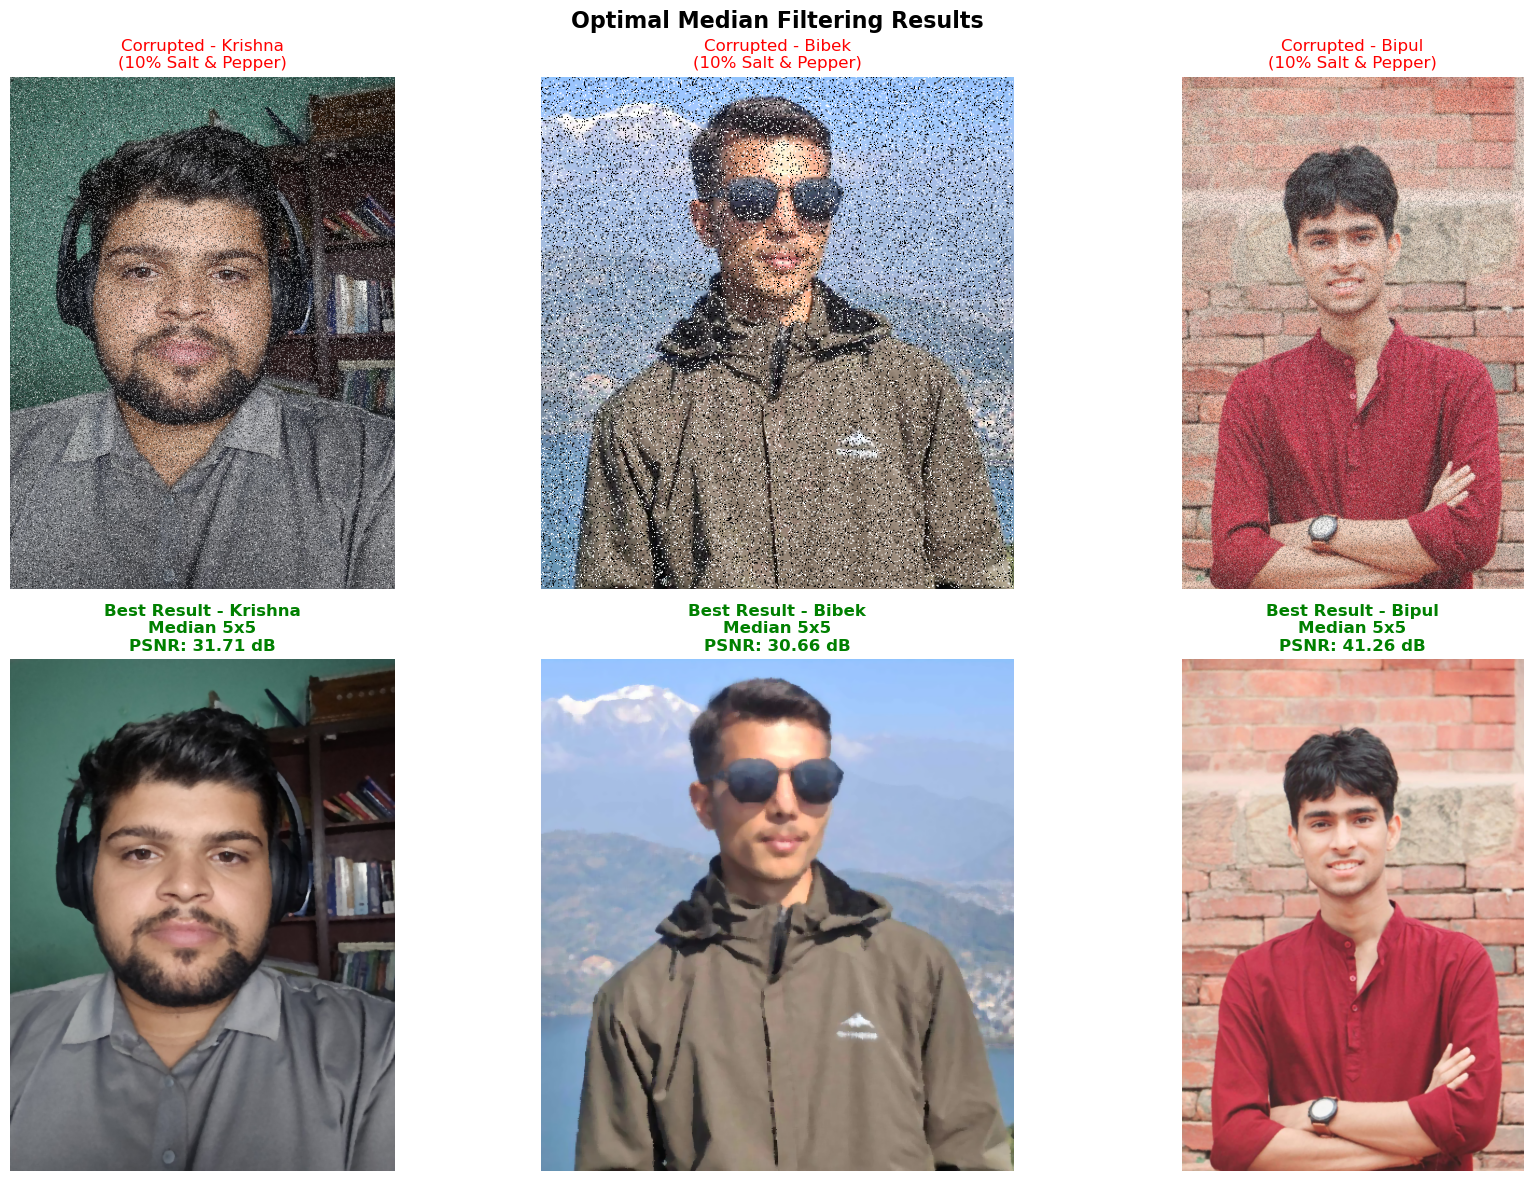
\includegraphics[width=0.5\textwidth]{img/outputs2/median_optimal.png}
    \caption{Optimal Median Filtering Results for 10\% Salt-and-Pepper Noise: The figure demonstrates the superior restoration quality achieved by the 5×5 median filter for images corrupted with 10\% salt-and-pepper noise. The results show excellent noise removal while maintaining fine image details and edge preservation.}
    \label{fig:median_optimal}
\end{figure}

\subsection{Median vs. Mean Filtering (Theoretical)}
While mean filtering was not implemented, the median filter is a non-linear operation that excels at preserving edges in images, making it highly effective for removing salt-and-pepper noise. It is robust to outliers and does not introduce new pixel values, resulting in minimal artifacts. However, it has moderate computational complexity. In contrast, the mean filter is a linear operation that tends to cause blurring and is generally ineffective against salt-and-pepper noise. It is sensitive to outliers and may introduce new pixel values, which can lead to averaging artifacts. On the positive side, the mean filter is computationally simple.

Morphological operations could provide alternative noise removal approaches. Opening operations remove small bright objects (salt noise) and preserve object boundaries using shape-based filtering, though they require careful structuring element design. Closing operations fill small dark regions (pepper noise), maintain object connectivity, and complement opening operations, making them particularly effective for binary image processing.

\subsection{Computational Performance Analysis}
Processing time measurements revealed the computational characteristics of different operations. Transformation complexity varies with reflection being O(n) and the fastest operation, while rotation and scaling operations have O(n) complexity with interpolation overhead. Shearing has O(n) complexity with moderate interpolation, and photometric operations have O(n) complexity for pixel-wise operations. Filtering complexity shows that median filtering has O(n × k²) complexity where k is kernel size, with 3×3 filters being fastest and 9×9 filters having the highest computational cost, demonstrating the trade-off between quality and speed.

\section{Conclusion}
This comprehensive laboratory investigation demonstrated the effectiveness of fundamental digital image processing techniques, including affine and non-affine geometric transformations, photometric augmentations, noise modeling, and restoration methods. Through systematic experimentation, the study highlighted how geometric operations such as rotation, reflection, shearing, and scaling enable robust manipulation of image structure, while photometric adjustments enhance visual quality without altering spatial relationships. The analysis of salt-and-pepper noise injection and subsequent restoration using median filtering revealed that a 5×5 kernel provides the best trade-off between noise removal and detail preservation, as confirmed by PSNR metrics. These findings underscore the importance of selecting appropriate transformation and filtering parameters to achieve optimal image quality, supporting a wide range of practical applications in computer vision, medical imaging, and automated systems.

The findings of this study have broad practical significance across multiple domains. In computer vision and machine learning, the demonstrated augmentation and restoration techniques enhance dataset diversity and model robustness, directly improving recognition accuracy and generalization. For medical imaging, effective noise removal and edge-preserving filtering contribute to higher diagnostic reliability and workflow efficiency. In surveillance and security, real-time image enhancement and geometric corrections support better identification and system calibration. Overall, the integration of these digital image processing methods enables more reliable, accurate, and efficient automated systems, facilitating advancements in both research and real-world applications.

\bibliographystyle{IEEEtran}
\bibliography{ref}

\end{document}
